\documentclass{beamer}
\usepackage[utf8]{inputenc}
\usepackage{mystyle} % See mystyle.sty for packages and own commands
\usepackage{dcolumn} % for aligning decimal points in table
\newcolumntype{d}[1]{D{.}{.}{#1}} % defining the column type
%------------------------------------------------------------
%Title page
\title[Sector and Industry Group Momentum]{Project Paper Digital Tools for Finance}
\subtitle{S\&P500 Sector and Industry Group Momentum}
\titlegraphic{
\includegraphics[height=2.0cm]{Logos/uzh_logo_e_pos_standard.png}}
\author[Fabian Mugrauer, Marco Bischoff]{
	Fabian Mugrauer,
	Marco Bischoff}
\institute[]{University of Zurich\\ Department of Banking \& Finance \\Igor Pozdeev}
\date{December 11, 2023}

%---------------------TITLE PAGE---------------------------------------
\begin{document}
\begin{frame}
\maketitle
\end{frame}
%------------------------------------------------------------

%-------------------------------------------------------------------

\begin{frame}
\frametitle{Table of Contents}
\tableofcontents
\end{frame}
%---------------------SLIDE---------------------------------------
\section{Intuition}
\begin{frame}{Intuition}    
\begin{itemize}
    \item Momentum is one of the most cited and strongest factors in academic literature and subject to many investment strategies in practice
    \item In our project we investigate whether a momentum setup as in \cite{jegadeesh1993returns} can be profitably applied in sector and industry group settings
        \begin{itemize}
            \item Sectors and industries are forms of combining companies with similar risk exposures into one basket
            \item Aggragating can help reduce transactions, reducing idiosyncratic risks while still preserving specific trend exposure evolving on a sector or industry level
        \end{itemize}
\end{itemize}
\end{frame}
%-------------------------------------------------------------------
\section{Backtesting Environment}
%---------------------SLIDE---------------------------------------
\begin{frame}{Backtesting Environment}
\begin{columns}[T] 

% Begin the left column
\begin{column}{0.45\textwidth} 
\begin{block}{Strategy Parameters} 
\begin{itemize}
    \item \textbf{Holding Period:} 3 months
    \item \textbf{Lookback Period:} 9 months
    \item \textbf{Rebalancing:} monthly
    \item \textbf{Long assets:} 3
    \item \textbf{Short assets:} 3
    \item \textbf{Transaction costs:} 10 BP (proportional)
    \item \textbf{Time Period:} September 1989 - October 2023
\end{itemize}
\end{block}
\end{column}

% Begin the right column
\begin{column}{0.45\textwidth} 
\begin{block}{Data} 
Daily data is downloaded from Bloomberg:
\begin{itemize}
    \item \textbf{Benchmark:} S\&P500 Total Return Index
    \item \textbf{Risk Free:} 3 Month T-Bill
    \item \textbf{Sectors:} S\&P500 Total Return GICS Sectors
    \item \textbf{Industry Groups:} S\&P500 Total Return GICS Industry Groups   
\end{itemize}
\end{block}
\end{column}

\end{columns}
\end{frame}

%-------------------------------------------------------------------

%-----------------------------SLIDE --------------------------------------
\begin{frame}{Long Only Momentum Performance vs. S\&P500}
    \centering % Center the image horizontally
    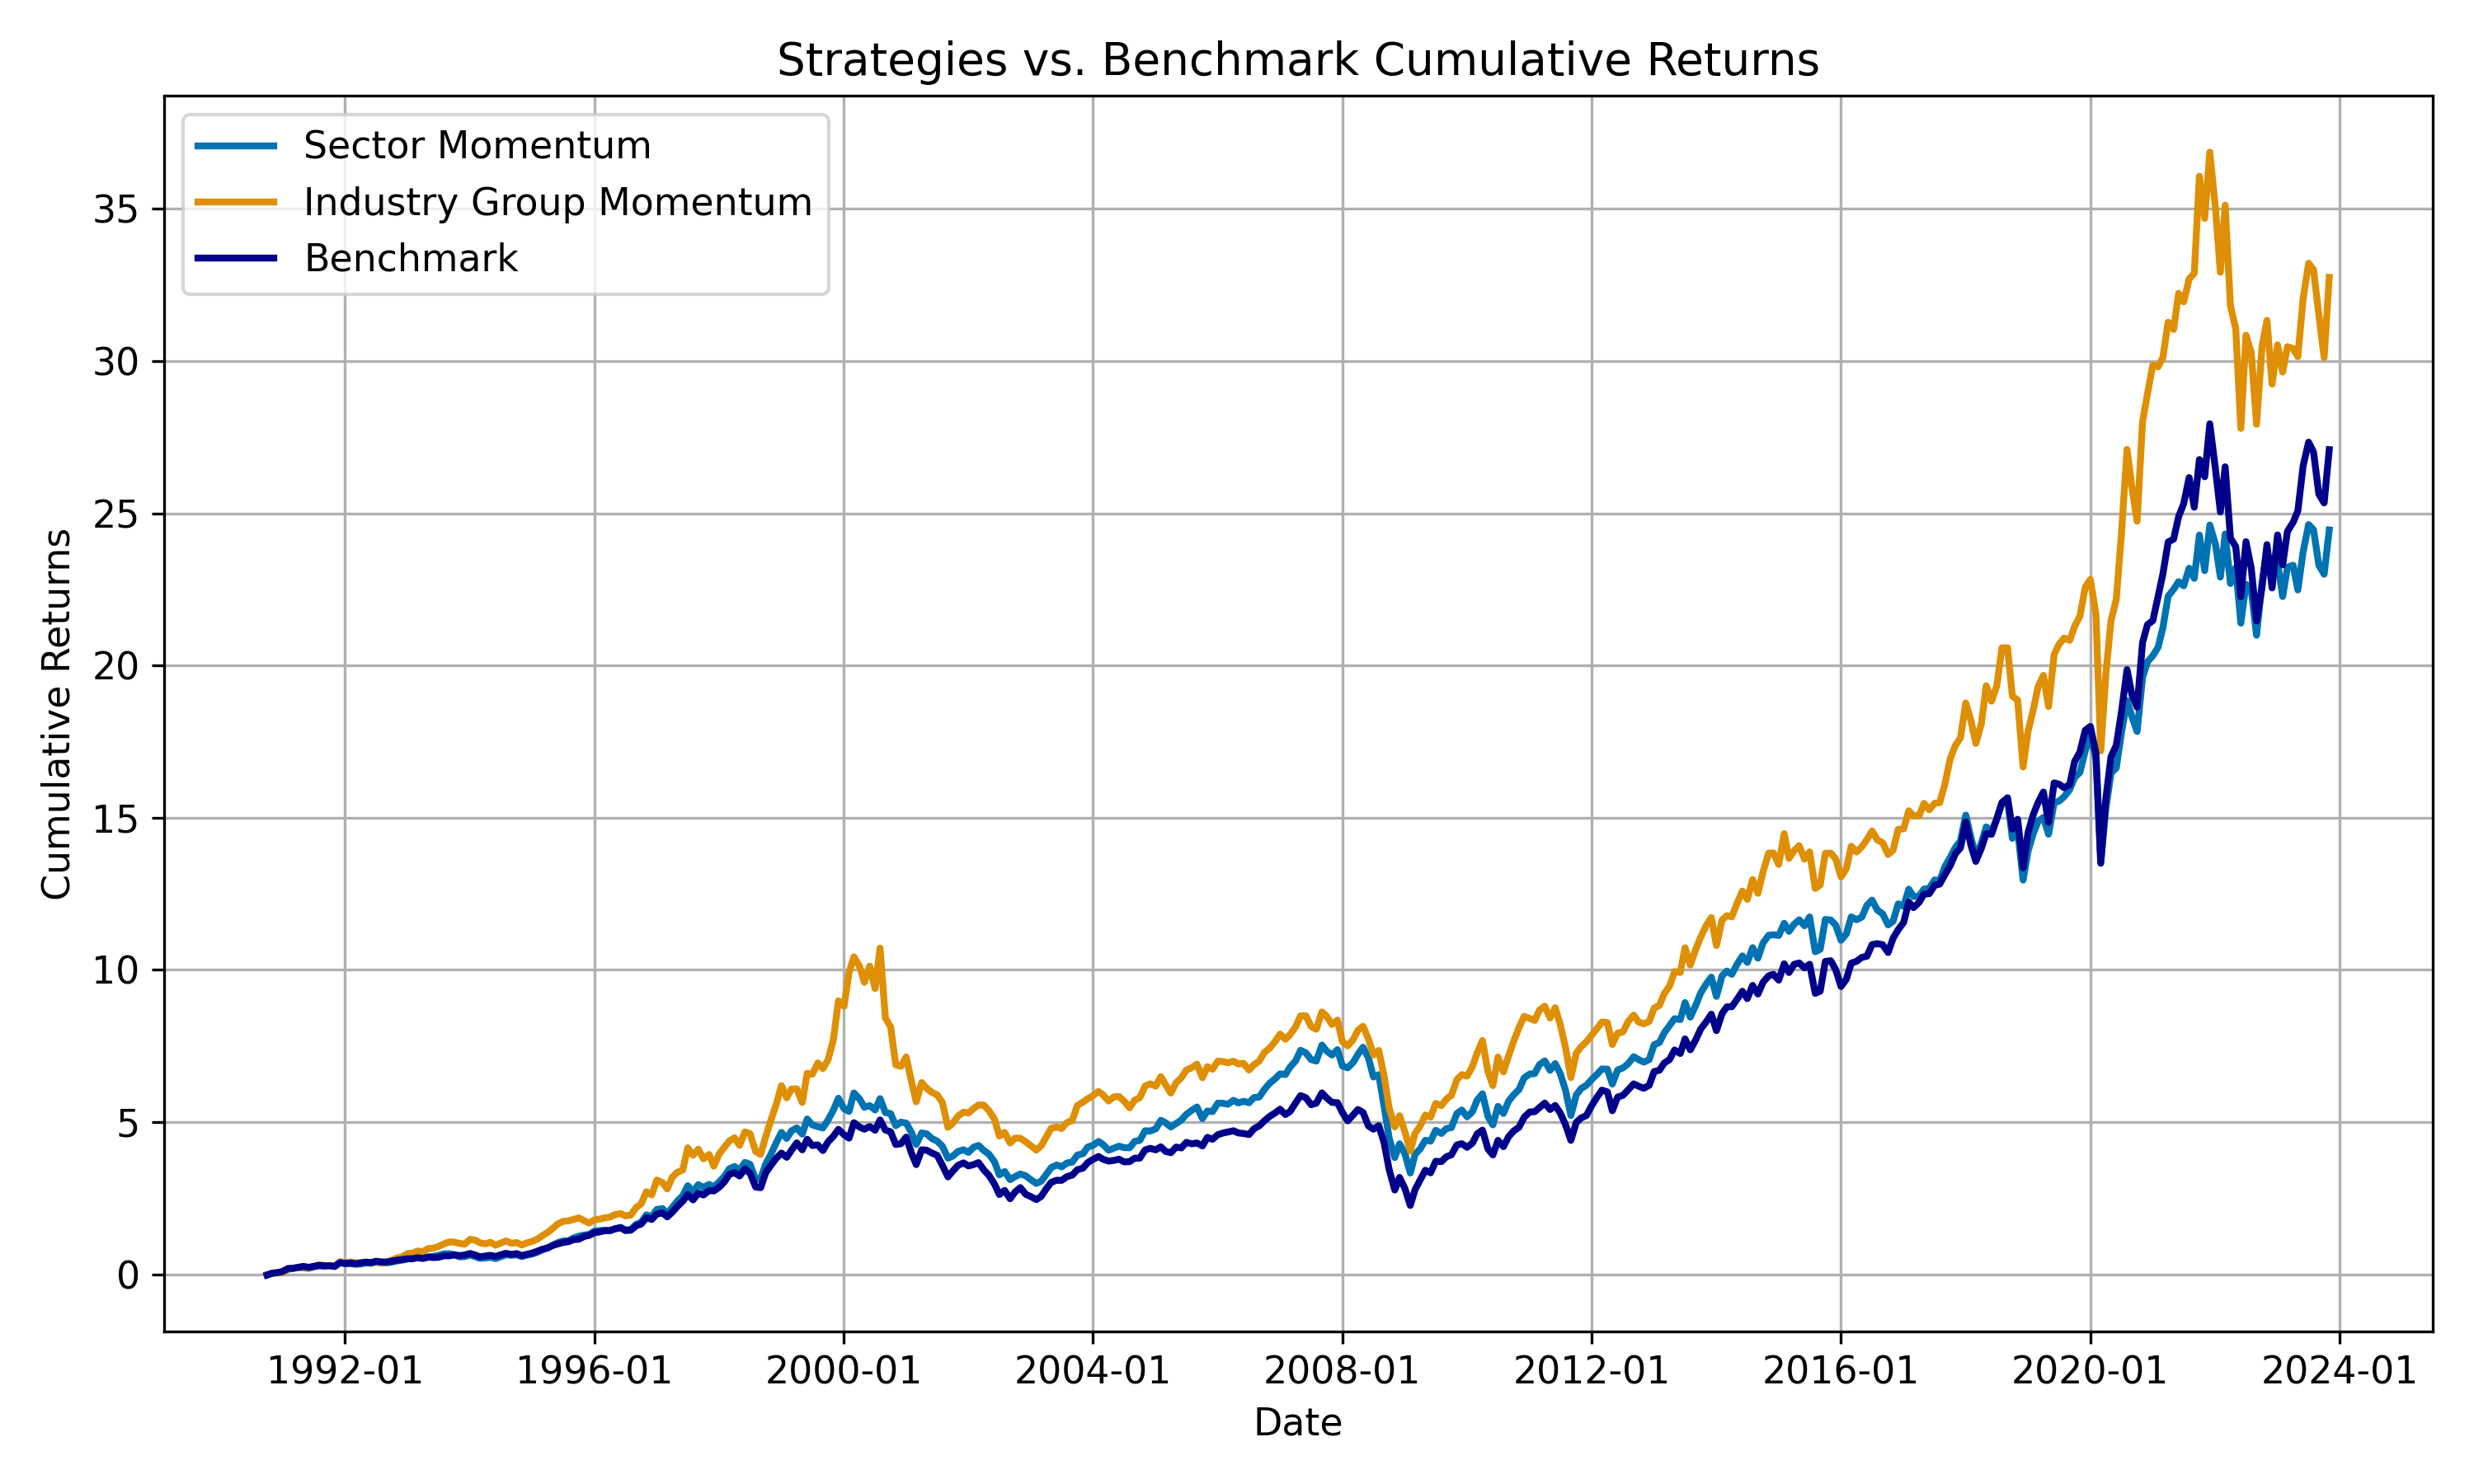
\includegraphics[width=1\textwidth]{Figures/strategy_plot.png}    

\end{frame}
%---------------------------------------------------------

%-----------------------------SLIDE --------------------------------------
\begin{frame}{Long/Short Momentum Performance vs. Risk Free Rate}
    \centering % Center the image horizontally
    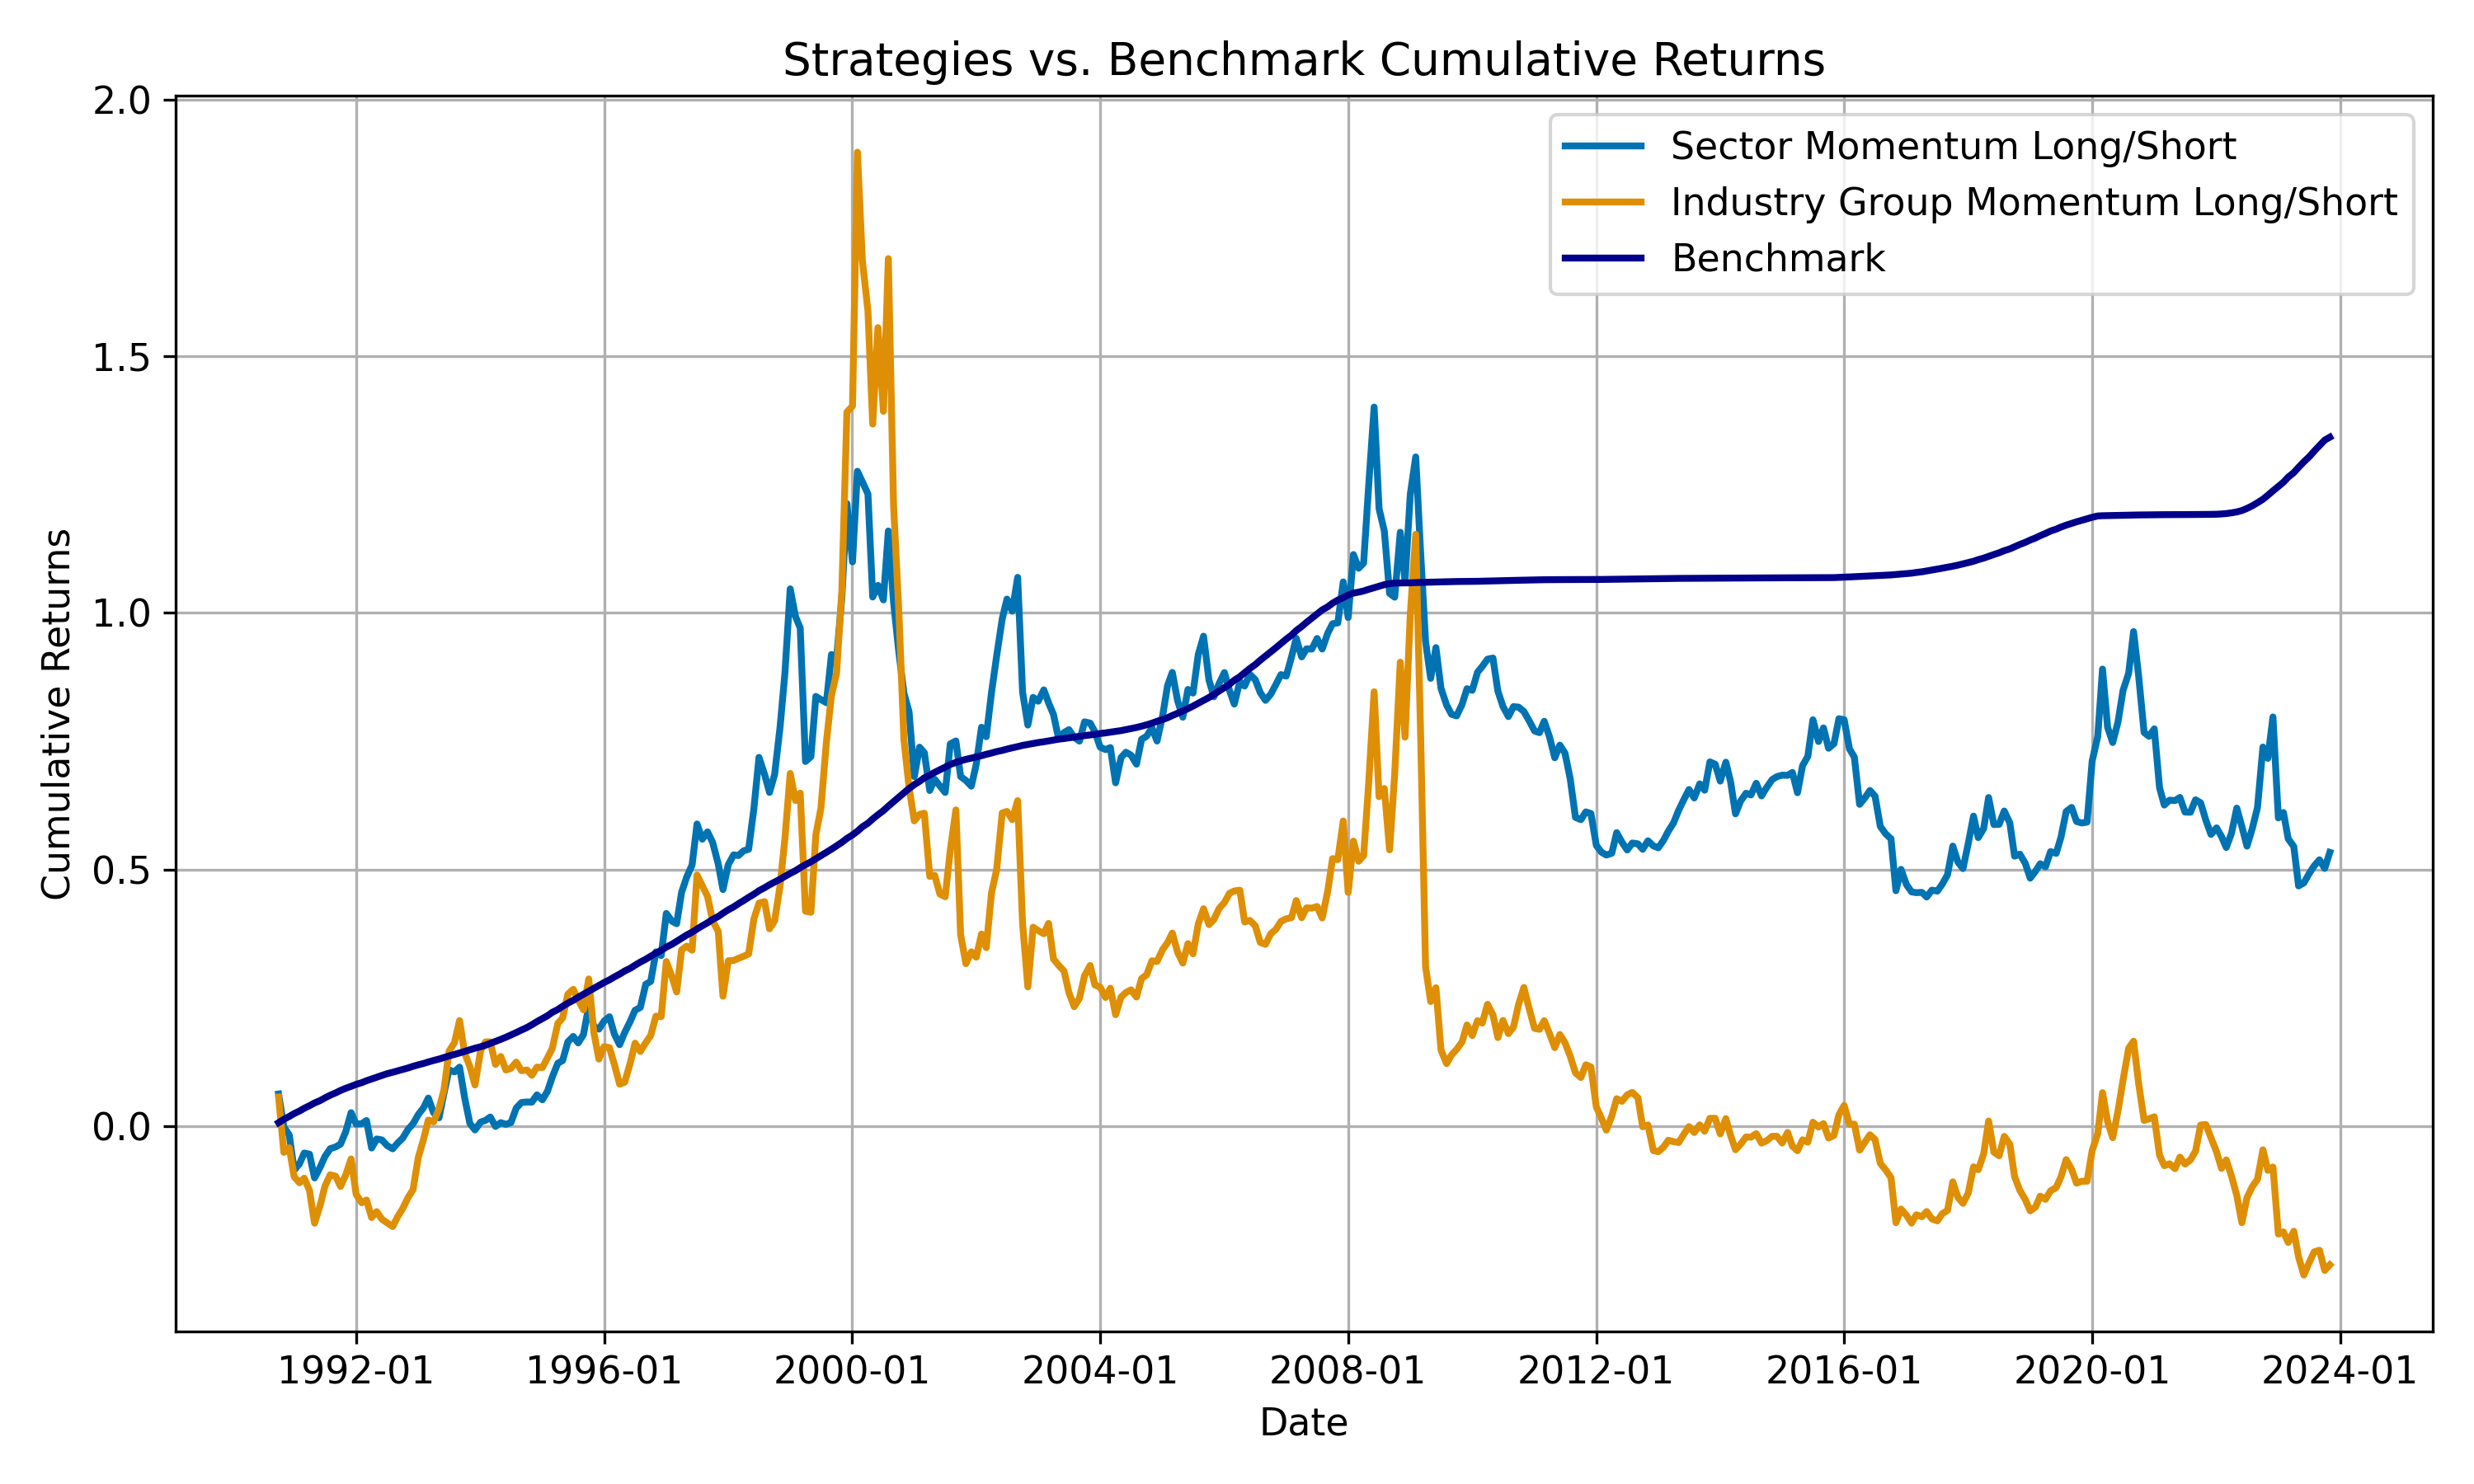
\includegraphics[width=1\textwidth]{Figures/strategy_plot_long_short.png}    

\end{frame}
%---------------------------------------------------------

%-----------------------------SLIDE --------------------------------------
\begin{frame}{Summary Statistics Sector and Industry Group Momentum vs. S\&P500}
    \begin{minipage}{\linewidth}
        \centering
        \begin{tabular}{@{\extracolsep{15pt}} ld{2.2}d{2.2}d{2.2}d{2.2}}
            \\[-1.8ex]\hline
            \hline \\[-1.8ex]
            & \multicolumn{2}{c}{Long only} & \multicolumn{2}{c}{Long/Short} \\
            \cline{2-3}\cline{4-5}
            & \multicolumn{1}{c}{Sectors} & \multicolumn{1}{c}{IG} & \multicolumn{1}{c}{Sectors} & \multicolumn{1}{c}{IG} \\
            \hline \\[-1.8ex] 
            Alpha & 0.33 & 0.52 & -2.07 & -3.35 \\
            (T-Value) & (0.35) & (0.35) & (-1.14) & (-1.20) \\
            Beta & 0.91 & 1.01 & 0.29 & -0.07 \\
            Excess Return & 8.38 & 9.71 & -0.72 & -2.14 \\
            Kurtosis & 1.82 & 1.32 & 2.05 & 4.38 \\
            Max & 14.14 & 16.01 & 8.58 & 20.13 \\
            Min & -18.81 & -20.09 & -13.59 & -26.19 \\
            STD & 15.03 & 17.96 & 10.52 & 16.41 \\
            Sharpe Ratio & 0.56 & 0.54 & -0.07 & -0.13 \\
            Skewness & -0.61 & -0.34 & -0.41 & -0.55 \\
            Total Return & 10.95 & 12.28 & 1.85 & 0.43 \\
           \hline
        \end{tabular}
    \end{minipage}
\end{frame}

%---------------------------------------------------------
\section{Robustness checks}
%-----------------------------SLIDE --------------------------------------
\begin{frame}{Net Sharpe Ratios vs.~Lookback Period for Long Only Sector and Industry Group Momentum Portfolios}
    \centering % Center the image horizontally
    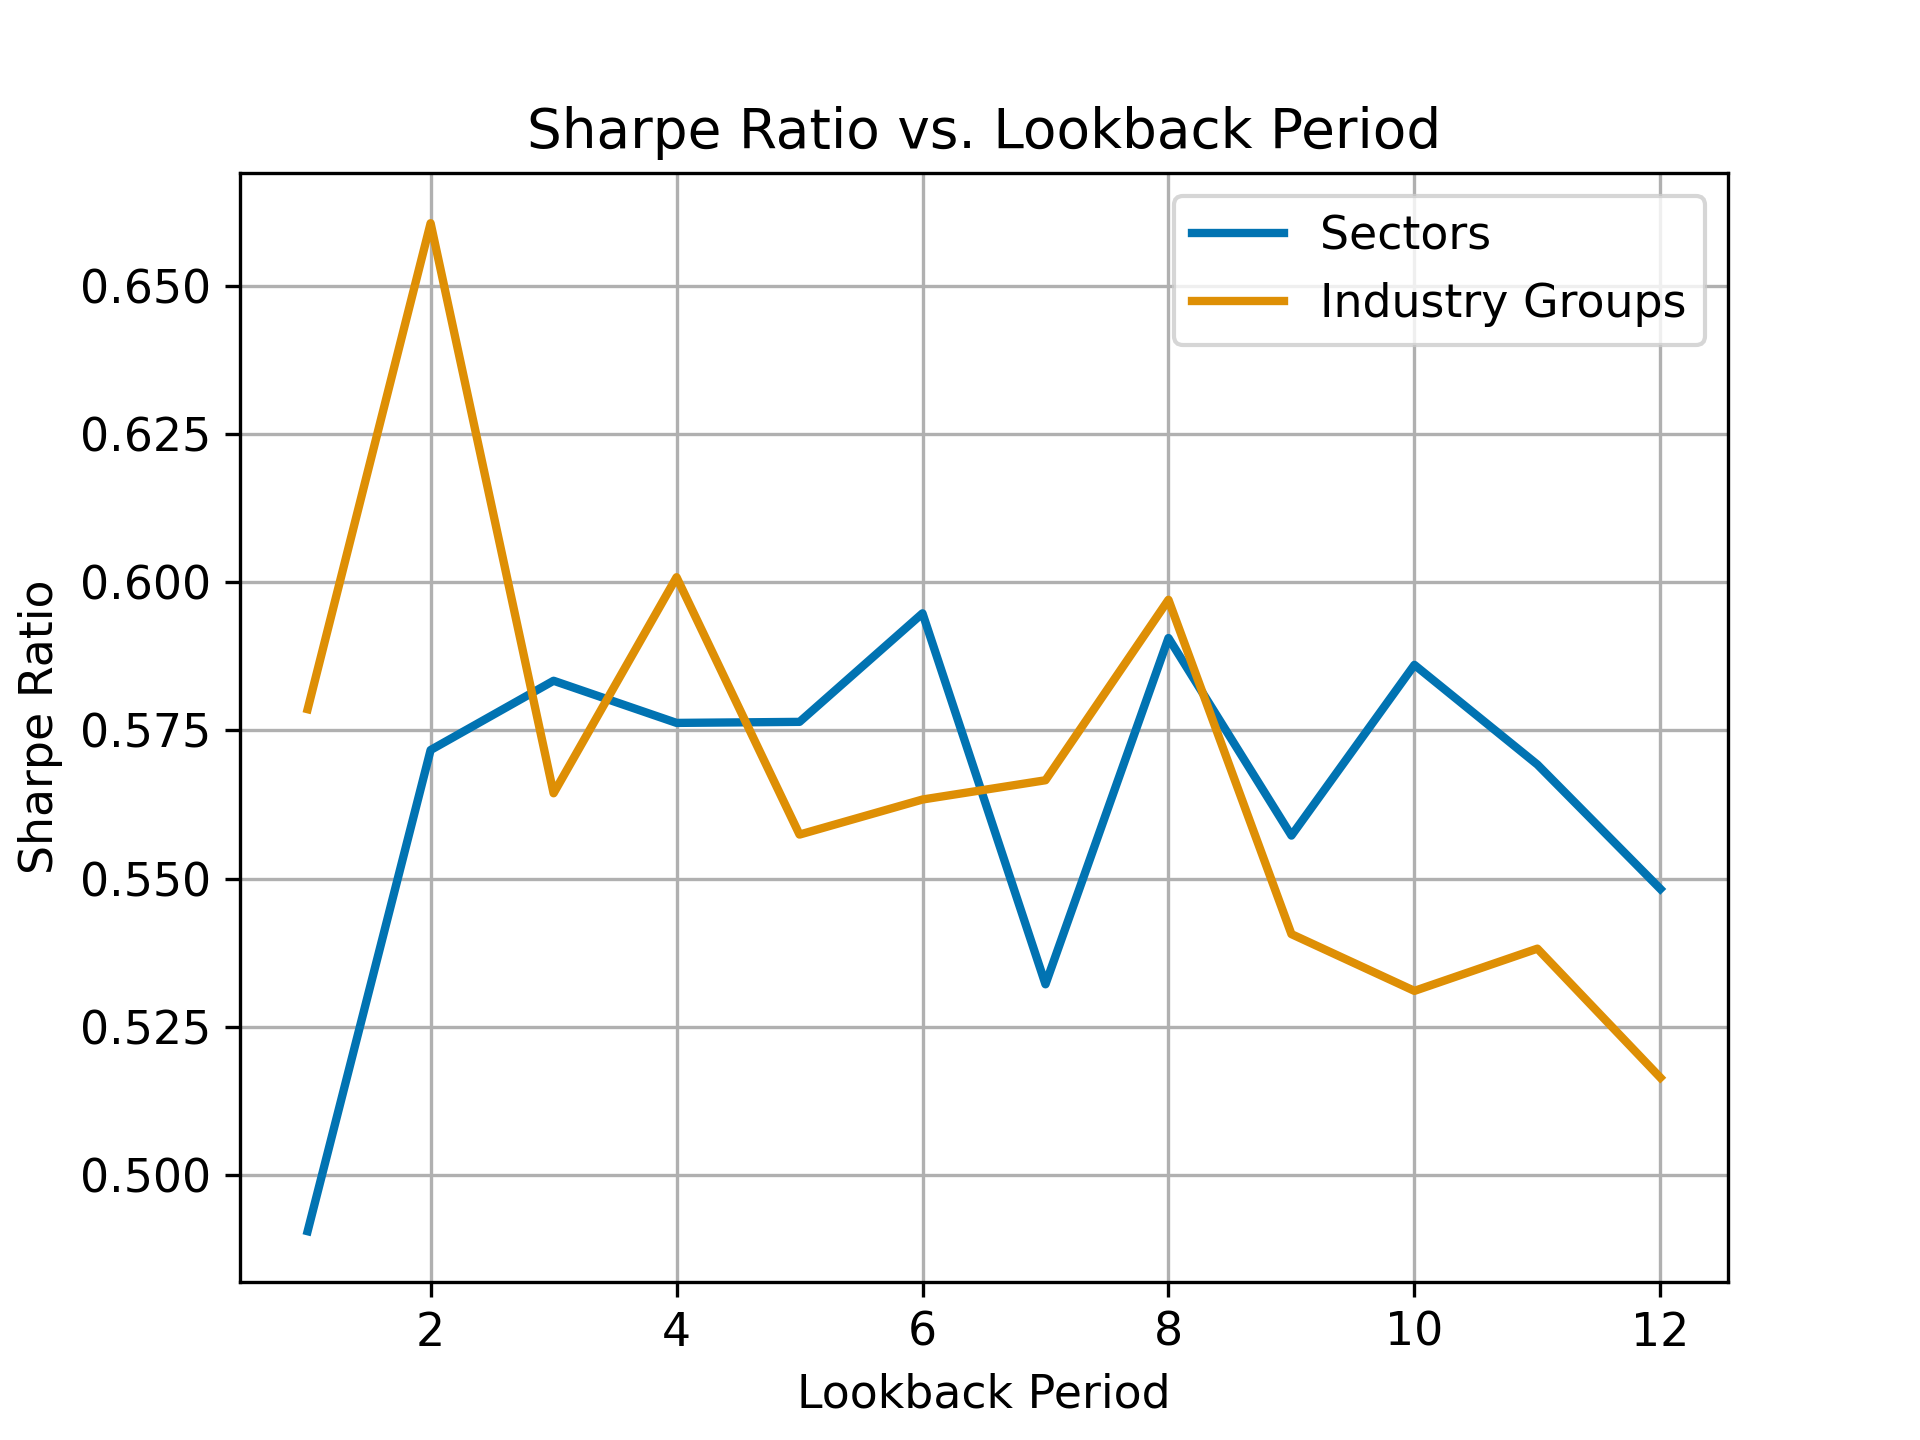
\includegraphics[width=0.8\textwidth]{Figures/robustness_check_lb.png}    

\end{frame}


%-----------------------------SLIDE --------------------------------------
\begin{frame}{Net Sharpe Ratios vs.~Holding Period for Long Only Sector and Industry Group Momentum Portfolios}
    \centering % Center the image horizontally
    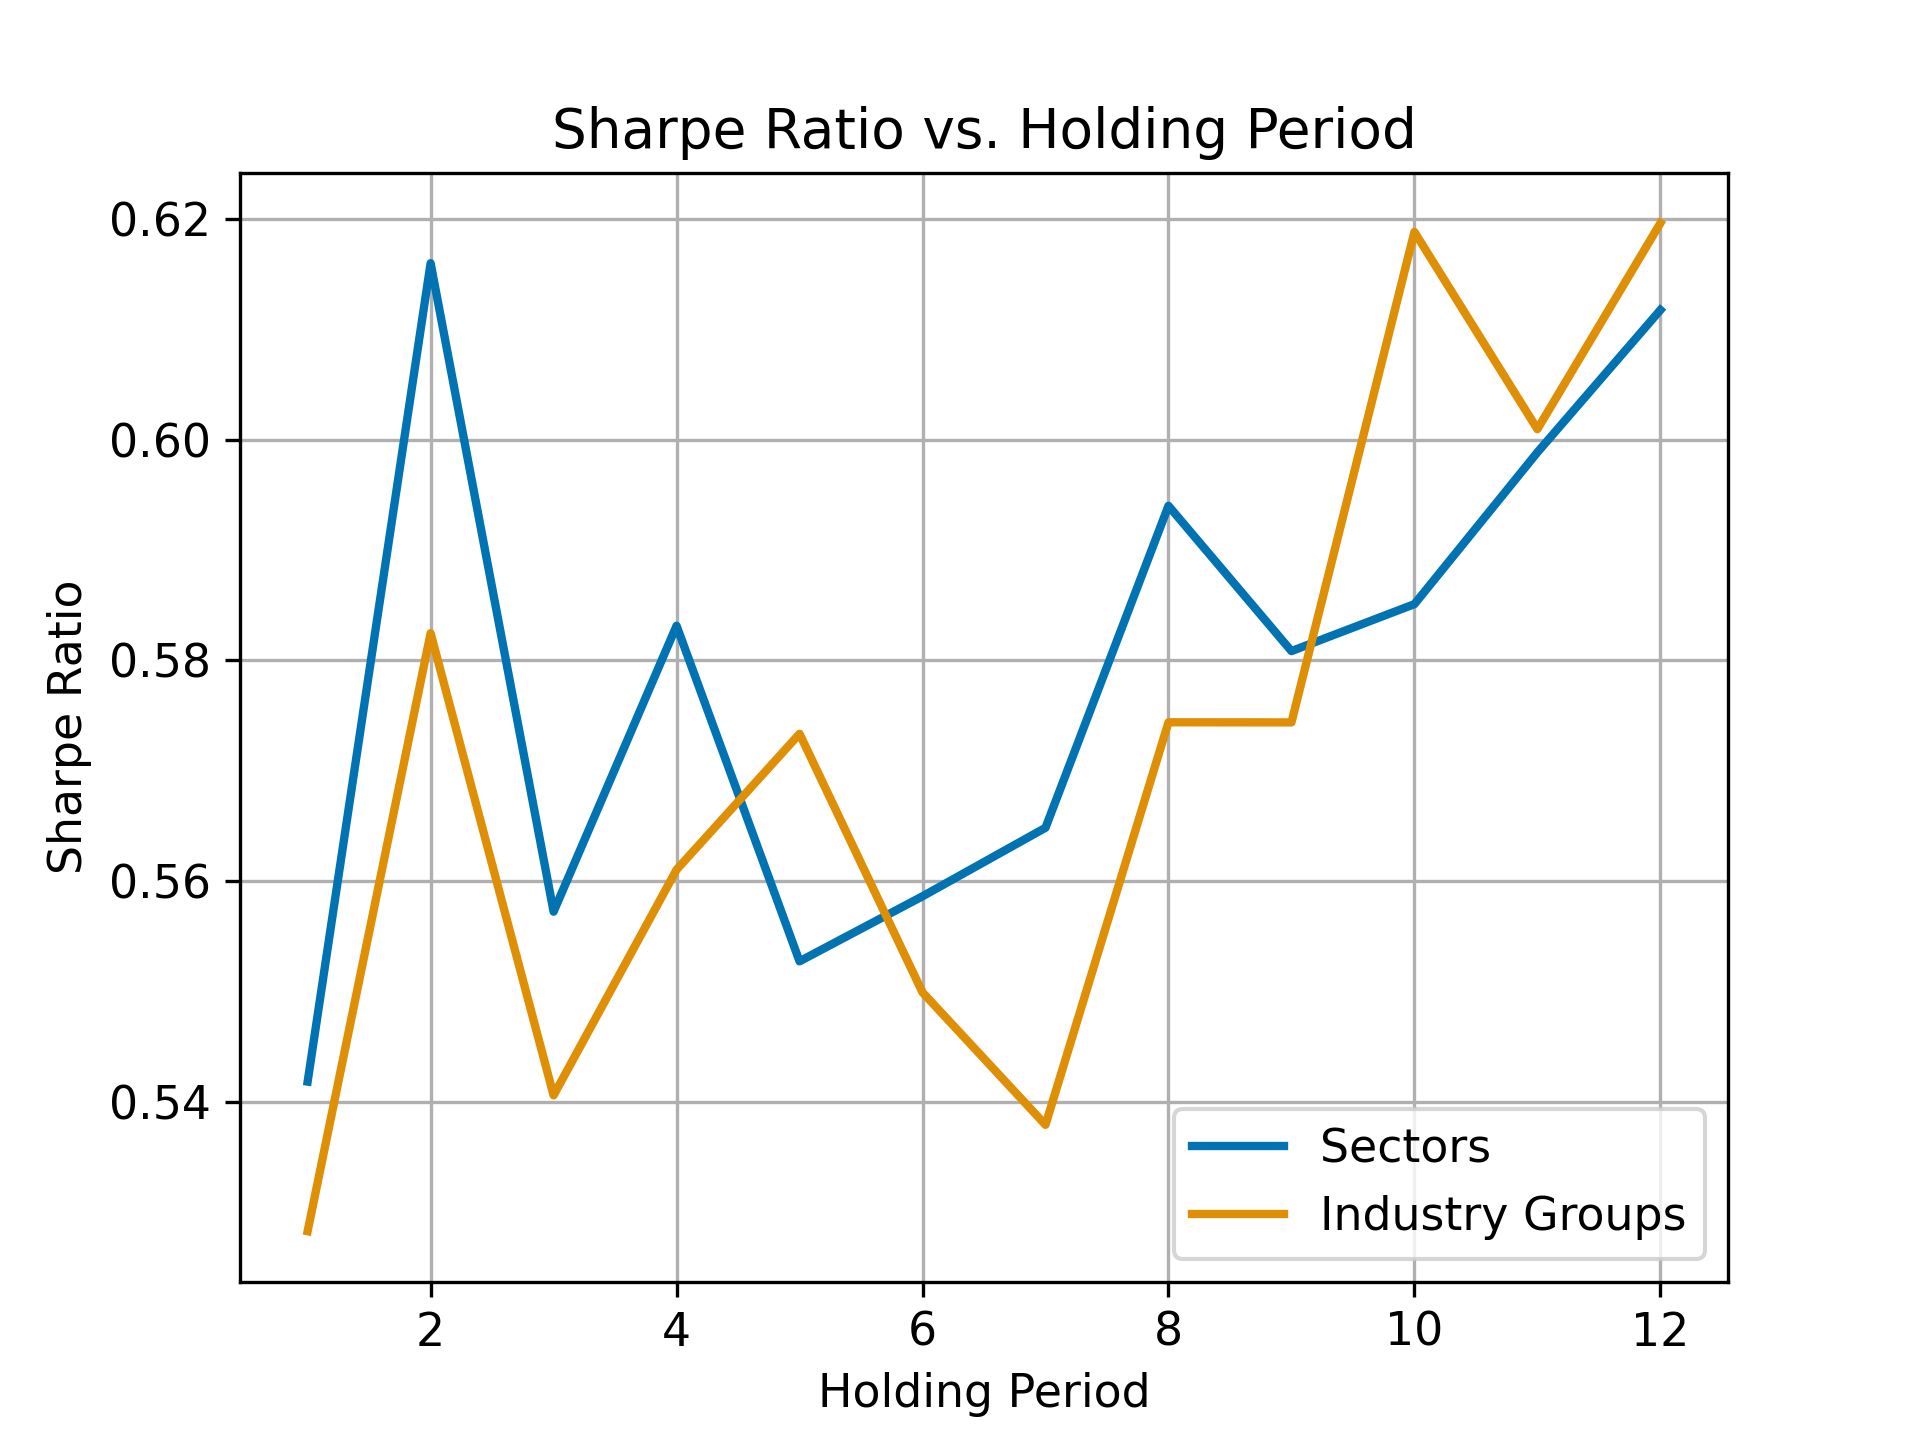
\includegraphics[width=0.8\textwidth]{Figures/robustness_check_ih.png}    

\end{frame}

%-----------------------------SLIDE --------------------------------------
\begin{frame}{Net Sharpe Ratios vs.~Number of Holdings for Long Only Sector and Industry Group Momentum Portfolios}
    \centering % Center the image horizontally
    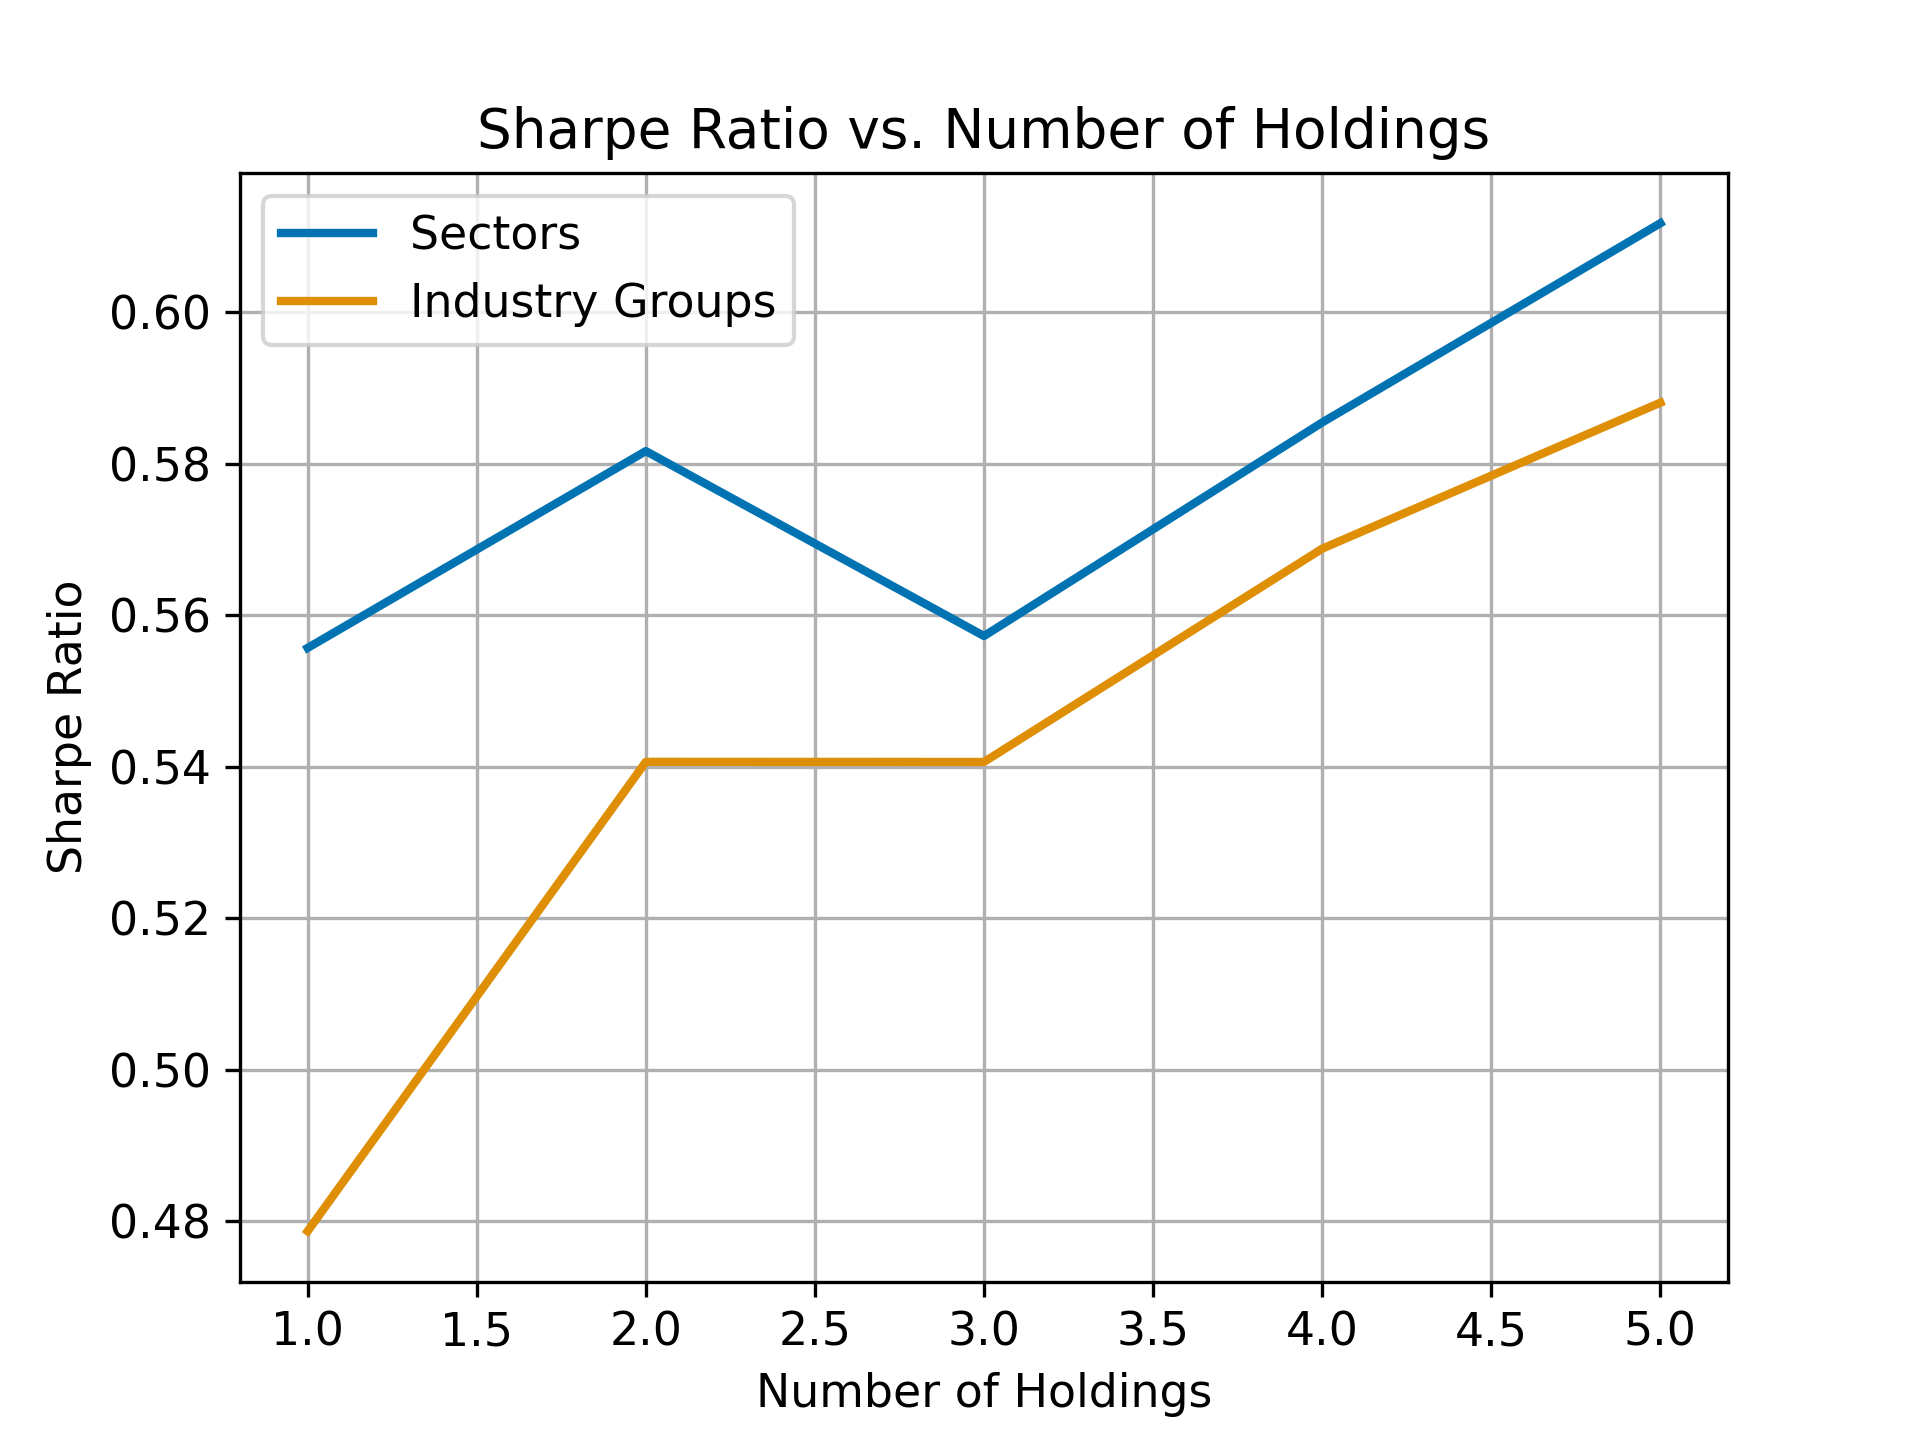
\includegraphics[width=0.8\textwidth]{Figures/robustness_check_holdings.png}    
\end{frame}

%-----------------------------SLIDE --------------------------------------
\begin{frame}{Net Performance vs.~Level of Transaction Costs for Long Only Sector and Industry Group Momentum Portfolios}
    \centering % Center the image horizontally
    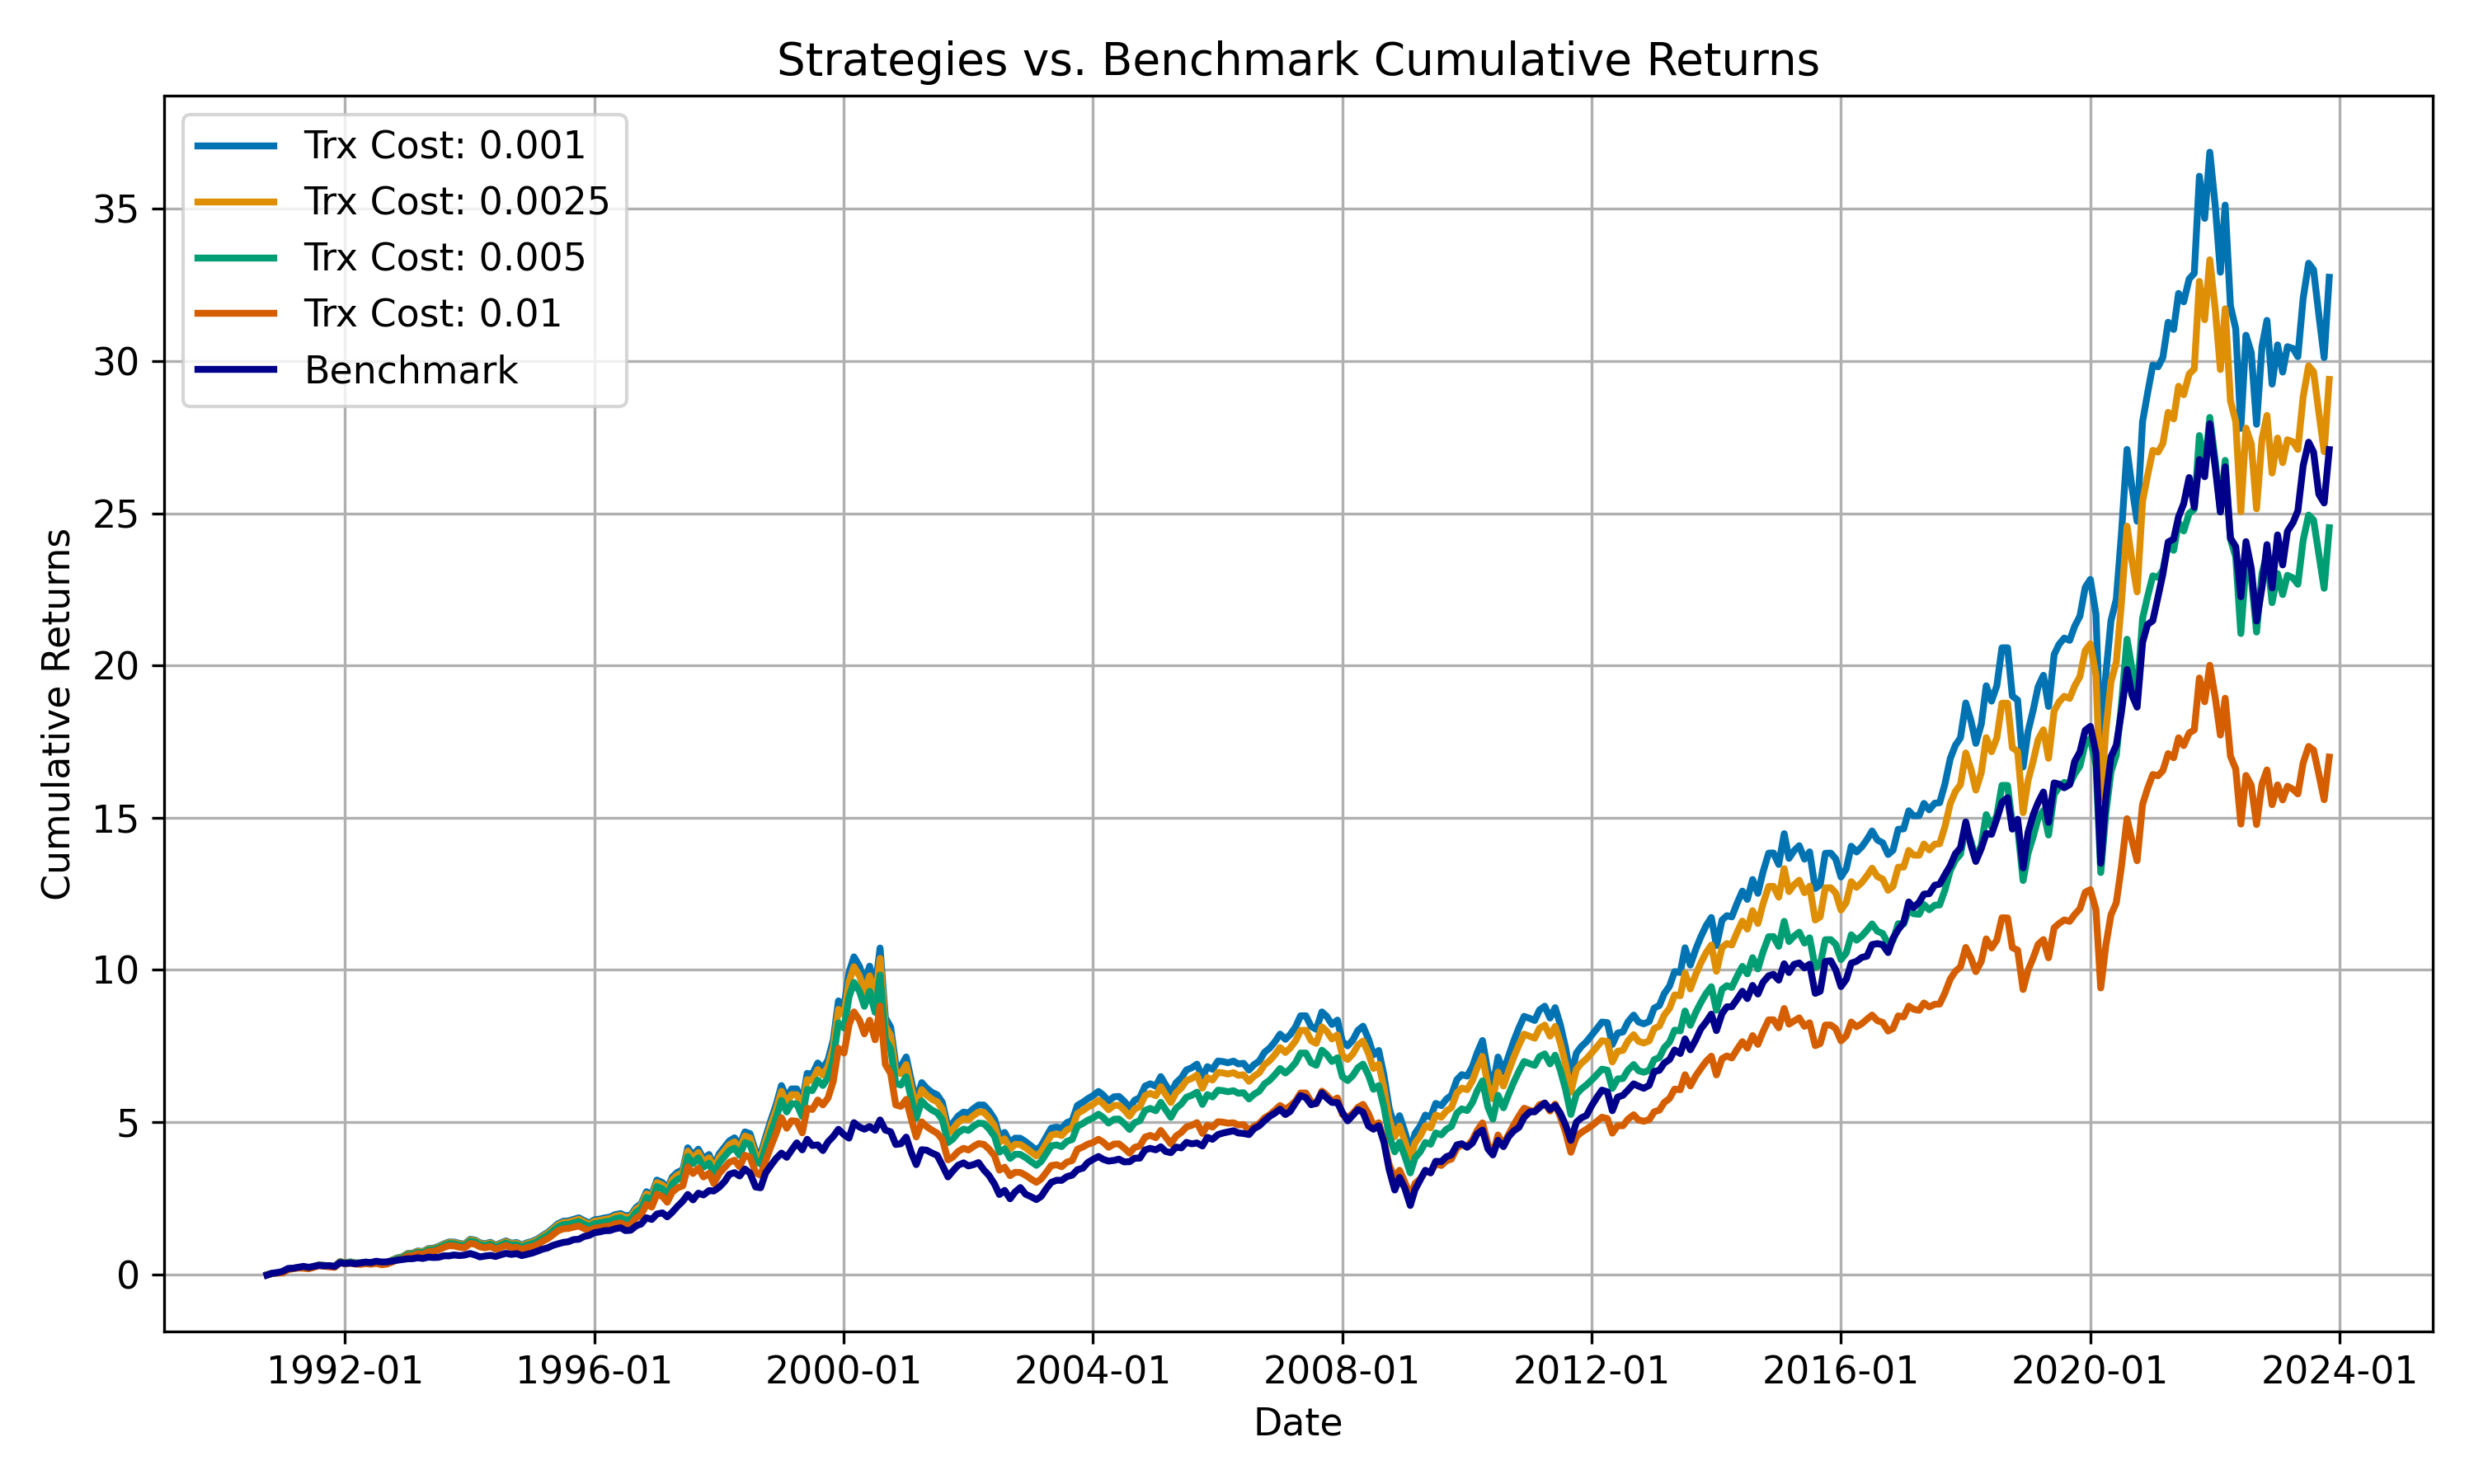
\includegraphics[width=1\textwidth]{Figures/robustness_check_tc.png}    
\end{frame}

\section{Conclusion}
%-----------------------------SLIDE --------------------------------------
\begin{frame}{Conclusion}    
\begin{itemize}
    \item We find that a pure long-only momentum strategy based on industry groups can generate excess returns
    \item A sector implementation did not work most likely because the level of aggragation is too high and thus the potential to generate alpha too low
    \item Including a short leg to exploit the UMD factor was a money losing strategy in the investigated period probably due to momentum crashes and is thus not attractive in real world settings
    \item Bottom line: The universe to select from plays a crucial role and is arguably more important then other input parameters.
    
    
    
\end{itemize}
\end{frame}



%---------------------------------------------------------


%---------------------------------------------------------
\section{References}
\begin{frame}[allowframebreaks]\frametitle{References}
        \bibliographystyle{apalike}
        \bibliography{bib}
\end{frame}


\end{document}